\documentclass{article}

\usepackage[spanish]{babel}
\usepackage{graphicx}
\usepackage{listings}
\usepackage{amsmath}

\begin{document}

% Titulo
%-------------------------------------------
\title{Informe Primer Proyecto de Programacion}
\author{Kevin Marquez Vega}
\date{Julio , 2023}

\maketitle

%-------------------------------------------
% Resumen
\begin{abstract}
    Para el desarrollo de este proyecto se nos encomendó la tarea de implementar un motor de búsqueda llamdo \textbf{Moogle}.
     A través de un \textbf{modelo vectorial} basado en \textbf{TF-IDF}, el programa recibe una consulta del usuario y devuelve los documentos
     más relevantes para dicha consulta de la base de datos que se encuentra en la carpeta \textbf{Content}.

     Cuenta además con varios operadores que permiten modificar los aspectos de la búsqueda y un sistema de sugerencias que
     en caso de no encontrar la palabra introducida por el usuario, realiza la búsqueda con la más semejante.
\end{abstract}

\newpage
\tableofcontents
\newpage
%-------------------------------------------
\section*{Estructura del Algoritmo}
El objetivo de implementar un modelo vectorial es representar tanto los documentos como la consulta como vectores, utilizando la fórmula de similitud
de coseno se podrá determinar cuales son más relevantes para la búsqueda y por tanto los que se deberán devolver al usuario.

Al comenzar la ejecución del programa es necesario cargar los documentos que componen la base de datos, estos son archivos
con extension ".txt" que se encuentran en la carpeta Content.

Para convertir un texto a vector es necesario determinar la "relevancia" de cada palabra dentro del documento como un valor numérico, quedando conformado
el vector por la unión de la relevancia de cada palabra que pertenezca a él.

Esa relevancia estará determinada por la fórmula del TF-IDF muy útil para esta tarea.

Una vez representados todos los documentos(y la consulta del usuario), el "score" de cada documento será determinado por la fórmula de similtud del coseno, la cual nos permite
determinar cuales documentos son los más relevantes.

Para terminar basta con devolver los documentos con mejor score, a través de un snippet que permita al usuario una breve lectura del documento.

No he incluido en esta estructura la ejecución de los operadores y la sugerencia, ya que se ejecutan en distintos momentos del flujo del programa, se pueden ver más 
detalladamente en la seccion : % REEEEEFFFFFFFFFFF

\begin{center}
    
\begin{figure}[ht]
    \label{fig : struct}
    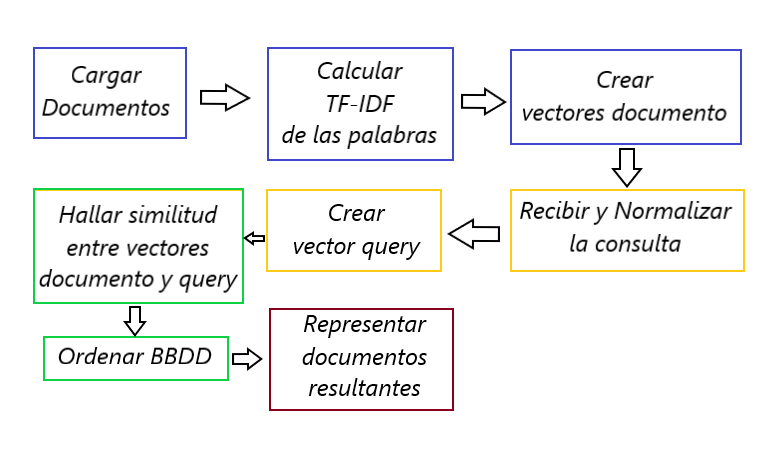
\includegraphics[width = 12cm]{./../images/struct.png}
    \caption{Estructura del algoritmo de Moogle}
\end{figure}
\end{center}

\newpage

\section{Representar documentos como vectores} \label{sec : vectores doc}

\subsection{Cargar documentos}\label{sec : load docs}
El programa debe ser capaz de acceder a la informacion de los documentos, es decir sus direcciones(ya sabemos que se encuentran en la carpeta Content).
La funcion \textit{SearchFiles} se encargara de esto, utilizando el metodo \textit{EnumerateFiles} de la clase \textit{Directory}.

\begin{lstlisting}[language={[Sharp]C} , basicstyle = \tiny]
    
public void SearchFiles(string dir)
{
    dir = Path.Combine(Directory.GetCurrentDirectory() , ".." , dir);
    IEnumerable<string> routes = Directory.EnumerateFiles(dir , "*txt" , SearchOption.AllDirectories);
        
    this.docs = new Document[routes.Count()] ;
        
    for( int i = 0 ; i < docs.Length ; i++)
    {
        // por cada ruta se crea un documento
        docs[i] = new Document(routes.ElementAt(i));
    }
}

    
\end{lstlisting}


Por cada ruta obtenida creamos objetos de la clase Documento, lo que nos permitira acceder a la informacion contenida en los archivos en cualquier momento.

\subsection{Crear vectores Documento} \label{sec : vd}

Ahora debemos crear los vectores Documento , donde cada término del vector será un valor numérico que representa la relevancia
de la palabra dentro del documento, conocido como \textit{tf-idf}.(Véase en la Seccion \ref{sec : tf-idf})

Para ello necesitamos dos datos : las veces que se repite cada palabra en cada documento y la cantidad de documentos donde aparece cada palabra

Surge entonces la siguiente interrogante : Cuál estructura de datos es mejor para almacenar dicha información ?

En este caso decidí utilizar un diccionario, ya que permite relacionar dos elementos en un par $<clave : valor>$ , las claves serán las palabras y
los valores otra estructura que guarde las veces que aparece dicha palabra en cada documento.

Mi primera idea para esa nueva estructura fue un array con el mismo \textit{Length} que el array de documentos de la base de datos.
De esa forma podria hacer coincidir el índice del documento con las veces que se encuentra la palabra en él.

Sin embargo, se necesitaría gran cantidad de memoria para almacenar todos esos datos y estarían compuestos por muchos 
ceros(de las palabras que no salen en el documento), los cuales no son relevantes.

Por esa razón decidí sustituir los arrays por diccionarios que relacionan el índice del documento con la cantidad de veces que posee la palabra,
sin necesidad de almacenar aquellos donde no se encuentre la palabra.

\begin{center}
    
\begin{figure}[ht]
    \label{fig : content}
    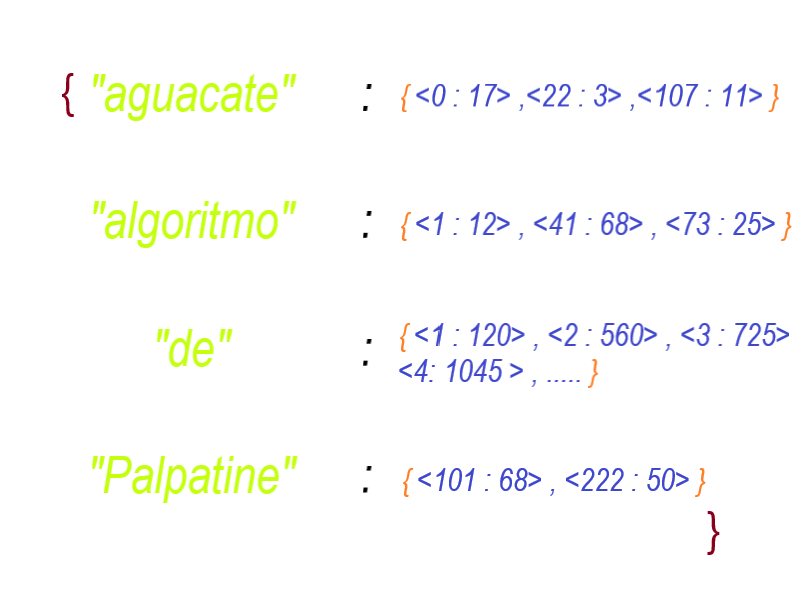
\includegraphics[width = 8cm]{./../images/content.png}
    \caption{Frecuencia de las palabras en los documentos}
\end{figure}

\end{center}

\section{Objetos tipo vector} \label{sec : vector}

El siguiente paso sería crear los vectores$(uno por cada documentos)$, intuitivamente pensaríamos que la mejor forma sería a través de un array, pero 
caeríamos en el mismo error de malgastar memoria.

Aplicando la misma idea, se podrian representar usando un diccionario donde a cada palabra se le hace corresponder el valor de su
\textit{tf-idf}.


\begin{figure}[ht]
    \label{fig : tfidf}
    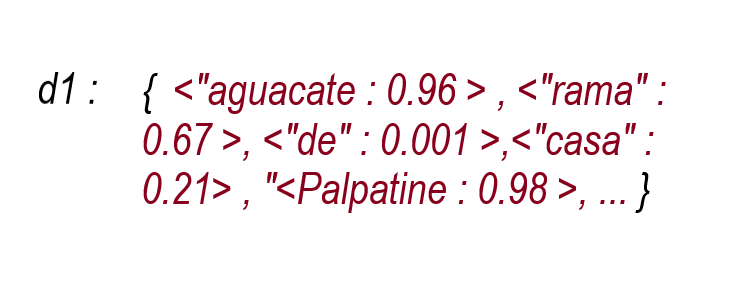
\includegraphics[width = 8cm]{./../images/tfidf.png}
    \caption{Vectores Documento}
\end{figure}

Hemos implementado un clase \textit{Vector} que tiene como propiedad ese diccionario, para poder añadir luego métodos que serán necesarios
en el trabajo con vectores.

De momento posee un indexer que facilita la entrada y salida de información de los vectores.

\section{Hallar TF-IDF} \label{sec : tf-idf}

Para calcular el \textit{tf-idf} de una palabra he utilizado las siguientes fórmulas : \\[1pt]

\begin{center}
    
$\text{TF-IDF} = TF \times IDF$ \\[10pt]

\begin{footnotesize}

\textit{\textbf{tf} : Term Frequency} \hspace{7pt}
\textit{\textbf{idf} : Inverse Document Frequency} \\[20pt]

\end{footnotesize}

$tf = \frac{n}{max_{fq}}$ \\[10pt]

\begin{footnotesize}

\textit{\textbf{n} : frecuencia de la palabra} \hspace{7pt}
\textit{\textbf{maxfq} : frecuencia de la palabra que más se repite} \\[20pt]

\end{footnotesize}


$idf = \log\frac{D + 1}{n_j + 1}$\\[10pt]

\begin{footnotesize}

\textit{\textbf{D} : total de documentos en la BBDD} \hspace{7pt}
\textit{\textbf{nj} : total de documentos donde aparece la palabra}   \\[20pt]

\end{footnotesize}

\end{center}

Luego, iterando sobre cada palabra en el diccionario Content, podemos obtener la cantidad de documentos donde aparece
la palabra usando dict.Count sobre el diccionario asociado a la palabra, el total de documentos de la base de datos sería 
docs.Length y así obtendríamos el \textit{idf}.

Para el \textit{tf} basta con iterar sobre las claves de ese diccionario relacionado a la palabra(que son los índices de los documentos
donde aparece la palabra), obtener la frecuencia de la palabra y utilizar ese índice para añadir el par \\$<palabra : tfidf>$
al vector del documento. \\[5pt]

\newpage

\begin{lstlisting}[language={[Sharp]C} , basicstyle = \footnotesize]
public void CreateVectors()
{
    Parallel.For(0 , docs.Length , i =>
    {
        docs[i].Vd = new Vector();

        int maxfq = Tools.MaxFq(Content , i) ; 
        foreach(string word in Content.Keys)
        {
            if(Content[word].ContainsKey(i))
            {
                double tf = Content[word][i] / (maxfq + 1.0) ;
                double idf = Math.Log10( (docs.Length + 1.0) / (Content[word].Count + 1.0) );
                docs[i].Vd[word] = tf * idf ;                
            }
                
        }
    });
}
\end{lstlisting}

\section{Representar la consulta como un vector}
Una vez representado cada documento como vector, faltaria recibir la consulta del usuario y transformarla en vector para
compararla con cada documento.


\subsection{Recibir y normalizar la consulta}
La consulta es recibida desde la interfaz gráfica del programa, un paso importante que debemos realizar es normalizarla.
Csharp es \textit{case-sensitive} , lo que significa que "casa" y "Casa" serán interpretadas como palabras diferentes cuando
en realidad es la misma.

Para evitar ese tipo de problemas, tanto los documentos como la consultan pasan por un proceso de normalización en el cual
se llevan todas las palabras a minúsculas, se eliminan caracteres extraños(excepto los operadores) y los espacios múltiples.

\subsection{Crear vector query}
Luego añadimos a la clase Base de Datos la propiedad Vq(vector query) que al igual que los vectores documentos será un diccionario
relacionando cada palabra con su \textit{tf-idf}.

Repitiendo el proceso de calcular el \textit{tf-idf}(esta vez sobre la consulta) podemos crear el vector query.

\section{Devolviendo resultados}
\subsection{Similitud entre vectores}
Una vez representados tanto los documentos como la consulta como vectores podemos calcular cuales son los más relevantes a partir
de la fórmula de similitud del coseno

\begin{center}
    
    $SimCos(A,B) = \frac{\sum_{i = 1}^{n}A_i  \cdot  B_i}{\sqrt{\sum_{i = 1}^{n}{A_i}^2} \cdot \sqrt{\sum_{i = 1}^{n}{B_i}^2}   } $\\[10pt]
    
\end{center}

El numerador es el producto escalar, que se obtiene multiplicando los términos con igual subíndice en ambos vectores(en mi interpretación 
los subíndices son las palabras). Notemos que si una palabra no forma parte del diccionario vector es porque su "relevancia" es 0
por tanto solo es necesario hallar el producto escalar con los valores de las palabras que se encuentren en ambos vectores.
\\[5pt]

\begin{lstlisting}[language={[Sharp]C}]
public static double EscalarProduct(Vector Q , Vector D)
{
    double suma = 0.0 ;
    foreach(string word in Q.v.Keys)
    {
        if(D.v.ContainsKey(word))
            suma += Q[word] * D[word];
    }
    return suma ;
}

\end{lstlisting}

El denominador esta determinado por la multiplicación de las normas de ambos vectores, la función \textit{GetNorma} nos devuelve
ese valor. \\[5pt]

\begin{lstlisting}[language={[Sharp]C}]
public double GetNorma()
{
    double suma = 0.0 ;
    foreach(double weigth in this.v.Values)
    {
        suma += Math.Pow(weigth,2);
    }
    return Math.Sqrt(suma);
}
\end{lstlisting}
    
Ambas funciones nos permiten hallar el \textit{score}(que estará entre 0 y 1), mientras más se acerque a 1, mas se acercará
a 0 la amplitud del ángulo que forman los vectores y por tanto será más relevante.

\subsection{Ordenar base de datos}
Ese valor de score lo guardaremos como una propiedad de cada documento, luego podemos ejecutar cualquier algoritmo de ordenación
sobre el array de documentos de la base de datos(en este caso utilicé Selection Sort).

Los primeros valores del array ordenado serán los documentos más relevantes.

\subsection{Representacion de documentos devueltos}
Una vez hallados estos documentos debemos devolver una porción de ellos donde aparezca alguna palabra de la consulta del usuario(snippet).

Para ello buscamos la palabra con mayor "relevancia" , esto es sencillo una vez tenemos el vector query. Esa será la palabra que 
aparecerá en el snippet y que llamaremos "pointerword".

Luego, con la función \textit{Find} encontraremos su primera aparición en el texto, devolviendo las diez palabras anteriores y posteriores(o el inicio/final del documento
en caso de que lo sobrepase).\\[5pt]


\begin{lstlisting}[language={[Sharp]C}]
string[] text = File.ReadAllText(this.route).Split();
int index = Tools.Find(pointerword , text);

int end = Math.Min(text.Length - 1 , index + 30);
for(int i = Math.Max(0, index - 10) ; i < end ; i++)
{
    snipe += text[i] + " " ;
}
return snipe ;

\end{lstlisting}


\section{Extras}
Este es el funcionamiento básico del Moogle, sin embargo poseía algunos requisitos adicionales como una serie de operadores
y una sugerencia en caso de encontrar pocos resultados

\subsection{Operadores}
Los operadores son simbolos que puede incluir el usuario que modifican la búsqueda, en esta version de Moogle se han implementado los operadores de
relevancia(*) , necesidad(\textasciicircum) y prohibición(!).


El primer problemas al que nos enfrentamos al incluir esta funcionalidad es que los operadores modifican la propia palabra
("**algoritmo" no coincidiría con "algoritmo") lo que haría que no se encontrase ninguna referencia a la palabra en la base de datos.

Para solucionar ese problema debemos cambiar la forma de recibir la consulta, en vez de un conjunto de palabras(string) creamos un objeto
tipo Term que tendrá dos propiedades : Text(la palabra) y mod(el modificador) almacenando el operador sin perder la funcionalidad del programa 
hasta el momento

\subsubsection{El operador de relevancia}
El operador de relevancia(*) al ser aplicado sobre una palabra indica que es más importantepara la búsqueda(se pueden añadir varios operadores * para
aumentar el efecto)

Para que haga efecto, al momento de calular el \textit{tf-idf} de la consulta se debe añadir una variable que represente la importancia(la cantidad de caracteres * en 
el modificador), por defecto su valor será 1 y por tanto no modificará el resultado, por cada * en la palabra el valor de
importancia aumentará en 1. \\[1pt]

$tf\textup{-}idf = tf \cdot idf \cdot imp$ \\[10pt]

\subsubsection{Los operadores de necesidad y prohibición}
Estos dos operadores tienen un funcionamiento similar, el operador de necesidad(\textasciicircum) obliga a que el documento devuelto posea la palabra que lo contenga.
De manera contraria, el operador de prohibición(!) obliga a que la palabra no aparezca en el documento.

Por lo cual, a la hora de calcular el score debemos chequear primeramente si cumple las condiciones del operador, en caso negativo su score será 0.
\\[5pt]

\begin{lstlisting}[language={[Sharp]C}]
public void GetScore(Vector Vq , Term[] terms)
{
    if(CheckIEOperators(terms))
        this.score = Vq * this.Vd ;
        
    else
        this.score = 0.0 ; 
}
\end{lstlisting}

Para chequear las condiciones basta con revisar el peso de la palabra en el vector documento. En el caso del operador de
necesidad el peso debe ser distinto de 0(ya que implica que la palabra está en el documento ) , entonces para el operador de prohibición
el peso debe ser igual a 0(la palabra no pertenece al documento). \\[5pt]

\newpage

\begin{lstlisting}[language={[Sharp]C} , basicstyle = \small]
private bool CheckIEOperators(Term[] terms)
{
    for(int i = 0 ; i < terms.Length ; i ++)
    {
        if(terms[i].Mod.Contains('^') && !this.Vd.v.ContainsKey(terms[i].Text))
            return false ;
            
        else if(terms[i].Mod.Contains('!') && this.Vd.v.ContainsKey(terms[i].Text))
            return false ;
    }
    return true ;
}    
\end{lstlisting}

\subsection{Sugerencia}
En caso que alguna palabra buscada por el usuario no aparezca en la base de datos o arroje pocos resultados, se podría añadir una funcionalidad que
le sugiera al usuario una palabra suficientemente parecida en su lugar, para ello utilizaremos una medida llamada \textit{Distancia de Levenshtein}

Esta distancia mide la diferencia entre dos cadenas de texto. Es el numéro mínimo de ediciones que se requieren para cambiar una cadena por otra. Las palabras
cuya distancia de Levenshtein sea menor serán las más parecidas y por tanto la que más probabilidades tenga de ser la buscada por el usuario.

Si el usuario introduce una palabra que no se encuentre en ningún, bastaría con encontrar la que menor \textit{Distancia de Levenshtein} posea con respecto
a ella y realizar la búsqueda con la nueva palabra, lo cual solucionaría por ejemplo los errores de escritura por parte del usuario ya que ¨aguqcatr¨ se transformaría
en "aguacate".

Para su cálculo me decidí por el método recursivo, ya que tarda menos que el iterativo, el cual luce así :
\newpage
\begin{lstlisting}[language={[Sharp]C} , basicstyle = \footnotesize]
// sobrecarga para que se vea mas bonito el llamado
public static int LevDistance(string a , string b) 
{
    int best = int.MaxValue ;
    LevDistance(a , b , 0 , 0 , 0 , ref best) ; // llamado feo
    return best ;
}

public static void LevDistance(string a ,string b ,int i ,int j ,int changes ,ref int best)
{
    if(changes > 3) {return ; }
    if(changes >= best) { return ; }

    while(i < a.Length && j < b.Length && a[i] == b[j])
    {
        i++ ;
        j++ ;
    }
        
    if( i >= a.Length || j >= b.Length - 1)
    {
        best = Math.Min( changes + (a.Length - i) + (b.Length - j) , best) ;
        return ;
    }
    
    LevDistance( a , b , i + 1 , j , changes + 1 , ref best) ;
    LevDistance( a , b , i , j + 1 , changes + 1 , ref best) ;
    LevDistance( a , b , i + 1 , j + 1 , changes + 1 , ref best) ;
}           
\end{lstlisting}


\end{document}